\documentclass[11pt]{article}

\usepackage[english]{babel}
\usepackage{authblk}
\usepackage[a4paper,top=2cm,bottom=2cm,left=2cm,right=2cm,marginparwidth=1cm]{geometry}
\usepackage{amsmath}
\usepackage{graphicx}
\usepackage{gensymb}
\usepackage{textcomp}
\usepackage[backend=biber, style=custom, maxcitenames=1, uniquelist=false, uniquename=false, url=false]{biblatex}
\usepackage{csquotes}
\usepackage[toc,page]{appendix}
\usepackage[colorlinks=true, allcolors=blue, breaklinks=true]{hyperref}
\usepackage{xurl}
\usepackage{multirow}
\usepackage{tabularx}
\usepackage{ltablex}
\usepackage{color}
\usepackage{tabularray}
\usepackage{indentfirst}
\usepackage{setspace}
\usepackage{orcidlink}

\doublespacing
\defbibenvironment{bibliography}
  {\begin{enumerate}}
  {\end{enumerate}}
  {\item}
\AtEveryBibitem{%
  \clearfield{note}%
}
\renewcommand\Affilfont{\itshape\centering}
\renewenvironment{abstract}{}{}
\newcommand{\keywords}[1]{
  \noindent\begin{center}\begin{minipage}{\textwidth}
  \small\textbf{Keywords:} #1
  \end{minipage}\end{center}
}
\DefineBibliographyStrings{english}{%
  andothers = {\textit{et al\adddot}},
}
\DeclareFieldFormat{doi}{%
  doi: \href{https://doi.org/#1}{\nolinkurl{#1}}%
}
\renewbibmacro*{doi+eprint+url}{%
  \iftoggle{bbx:doi}
    {\printfield{doi}}
    {}%
  \newunit
  \iftoggle{bbx:eprint}
    {\usebibmacro{eprint}}
    {}%
  \newunit
  \iftoggle{bbx:url}
    {\usebibmacro{url+urldate}}
    {}}

\addbibresource{references.bib}

\title{Estimating Ensemble Location and Width in Binaural Recordings of Music with Convolutional Neural Networks}
\author[1,*]{Paweł Antoniuk\orcidlink{0000-0002-0914-8920}}
\author[1]{Sławomir K. Zieliński\orcidlink{0000-0002-3205-974X}}
\affil[1]{Faculty of Computer Science, Białystok University of Technology \protect\\ Wiejska 45A, 15-351 Białystok, Poland}
\affil[*]{Corresponding Author Email: pawel.antoniuk@sd.pb.edu.pl}
\date{}

\begin{document}

\maketitle

\begin{abstract}
  Binaural audio technology has been in existence for many years. However, its popularity has significantly increased over the past decade as a consequence of advancements in virtual reality and streaming techniques. Along with its growing popularity, the quantity of publicly accessible binaural audio recordings has also expanded. Consequently, there is now a need for automated and objective retrieval of spatial content information, with ensemble location and width being the most prominent. This study presents a novel method for estimating these ensemble parameters in binaural recordings of music. For this purpose, a dataset of 23,040 binaural recordings was synthesized from 192 publicly-available music recordings using 30 head-related transfer functions. The synthesized excerpts were then used to train a multi-task spectrogram-based convolutional neural network model, aiming to estimate the ensemble location and width for unseen recordings. The results indicate that a model for estimating ensemble parameters can be successfully constructed with low prediction errors: $4.76\degree$ ($\pm0.10\degree$) for ensemble location and $8.57\degree$ ($\pm0.19\degree$) for ensemble width. The method developed in this study outperforms previous spatiogram-based techniques recently published in the literature and shows promise for future development as part of a novel tool for binaural audio recordings analysis.
\end{abstract}

\keywords{ensemble width, ensemble location, binaural, spatial audio, localization, convolutional neural network, head-related transfer function, angle of arrival}

\section{Introduction}

The human auditory system demonstrates exceptional proficiency in segregating, localizing, and interpreting diverse auditory signals, despite being limited to two ears. This is possible, among other factors, by internal examination of interaural differences in time, loudness, and frequency, known as binaural hearing \parencite{blauert_spatial_1996}, which enables precise localization of sound sources in complex auditory environments. A notable advantage of binaural hearing is exemplified by the ``cocktail party effect'', highlighting humans' capability to concentrate on foreground sound sources while suppressing background noise \parencite{cherry_experiments_1953}. Understanding of the auditory system is essential for comprehending its limits but also for leveraging these insights to create more immersive binaural experiences for entertainment purposes \parencite{zhang_surround_2017}. It is also important for enhancing auditory signal reception in hearing aid devices \parencite{hirsh_binaural_1950, thiemann_speech_2016}.

The advance of sophisticated machine learning techniques, especially deep learning networks, has initiated an interesting exploration of their potential to emulate the human auditory system. Recently emerged studies have demonstrated that relying on the advanced spatial audio feature engineering is not necessary in computational audio source localization \parencite{vera-diaz_towards_2018, pang_multitask_2019, yang_deepear_2022}. While applying convolutional neural networks (CNNs) \parencite{lecun_handwritten_1989} to audio signals is well-established, often in conjunction with spectrograms \parencite{thomas_analyzing_2014, espi_exploiting_2015, han_convolutional_2017} or other feature engineering techniques \parencite{abdel-hamid_applying_2012, sainath_deep_2013}, these approaches continue to be refined and adapted for audio processing. Building on these foundations, this study develops an audio localization method using a spectrogram-based multi-task CNN model.

Humans tend to localize groups of sound sources rather than individual ones \parencite{bregman_auditory_1990, rumsey_spatial_2002}. Inspired by this fact, the objective of the proposed model is to estimate the location and width of these groups, termed ``ensembles,'' instead of the positions of individual sources. This study is unique as it not only developed the method but also tested it on a relatively large, realistic music corpus. The corpus comprised 23,040 binaural excerpts synthesized using 192 multi-track music recordings (from a repository provided by \textcite{senior_mixing_2023}) and 30 sets of publicly available head-related transfer functions (HRTFs) acquired from various sources (see Table \ref{table:hrtfs} in \nameref{appendix:a_hrtf} for a detailed list). The music recordings covered many different genres, including rock, jazz, pop, and classical music.

The findings demonstrate that this method is effective in accurately estimating the spatial characteristics of groups of sound sources in near-real-world scenarios. This paper also demonstrates an experimental framework that facilitates the objective measurement of a binaural localization technique, employing a large-scale dataset synthesized from real-world music signals (for applications of similar frameworks, see studies conducted by \textcite{antoniuk_blind_2023, zielinski_automatic_2022, zielinski_spatial_2022, zielinski_comparison_2020}). One of the key advantages of the proposed method is that it does not assume the number of audio sources. However, significant limitations of this study include the absence of reverberation in the synthesized recordings and the method's inapplicability to real-time scenarios --- both are critical areas for future research.

The developed method has the potential to be highly beneficial in automated information retrieval tasks, where a significant number of binaural recordings must be analyzed or labeled in terms of their spatial content information. This could be utilized in the development of a hypothetical autonomous ``web-crawler bot'' that will collect binaural recordings from publicly accessible repositories and label them according to the spatial properties of the sound sources, such as the location of the music ensemble or the sparsity of audio source positions. This method may also assist audio engineers in objectively assessing and segregating binaural audio recordings with regard to their spatial content.

This paper is structured as follows: Section \ref{sec:related-studies} presents related studies. The description of the method developed for this study is provided in Section \ref{sec:methodology}, which also includes detailed definitions of ensemble location and width, along with a description of the experiments used to evaluate this method. Section \ref{sec:results} presents and discusses the performance of the proposed method as well as the results of the experiments conducted in this study. Finally, Section \ref{sec:conclusions} offers concluding remarks and suggestions for future research.

\section{Related studies}
\label{sec:related-studies}

Most existing literature on computational sound source localization reports techniques that take advantage of multiple microphone arrays with more than two channels \parencite{kaveh_statistical_1986, pavlidi_real-time_2012, pan_multi-tone_2021, hahmann_sound_2022, chung_sound_2022, liu_sound_2022}. Although these methods can improve localization precision by providing additional spatial information, they do not utilize binaural hearing, rendering them ineffective for binaural recordings. In the context of sound source localization in binaural signals, the  focus of research is put on the identification of individual sound sources, rather than groups of sounds \parencite{dietz_auditory_2011, may_probabilistic_2011, may_binaural_2012, woodruff_binaural_2012, may_robust_2015, ma16c_interspeech, ma_exploiting_2017, benaroya_binaural_2018}.

Considering source Direction of Arrival (DoA) methods, the majority of research assumes a fixed number of sound sources \parencite{pang_multitask_2019, vera-diaz_towards_2018, ma_exploiting_2017, woodruff_binaural_2012, arthi_spatiogram_2021}, which limits its practical applications as this information is rarely known in real-life binaural recordings. Moreover, the majority of studies have focused on relatively homogeneous signals, namely speech \parencite{dietz_auditory_2011, may_probabilistic_2011, may_binaural_2012, woodruff_binaural_2012, may_robust_2015, ma16c_interspeech, ma_exploiting_2017, benaroya_binaural_2018, wang_binaural_2020, liu_multiple_2018, yang_deepear_2022, ma_robust_2018}.

In contrast to the aforementioned studies, the proposed method is not constrained by the number of sources. Moreover, the approach is not narrowed to speech and has been applied to a wide range of musical datasets, including instruments and vocals. In contrast to studies that primarily focused on individual sources, the proposed method does not aim to separate them, but rather considers them as a group, or in this case --- a musical ensemble --- similar to how real musical ensembles are arranged on stage. To the authors' knowledge, this is one of the first methods to localize ensemble width (see \textcite{antoniuk_blind_2023} for the previous ensemble-width-related study), and the first to localize both ensemble position and width simultaneously using a multi-task model.

Sound localization methods can be classified into two categories based on the implementation of their underlying algorithms, termed as glass-box and black-box techniques. Glass-box methods could be considered as more traditional in the literature. They rely on manually designed algorithms that mimic the auditory system to explicitly extract key features for the localization estimation, such as interaural level differences, interaural time differences, interaural coherence, or interaural phase differences (\textcite{blauert_spatial_1996} provides detailed descriptions of these features). Examples of glass-box methods can be found in numerous studies, including those conducted by \textcite{dietz_auditory_2011, may_probabilistic_2011, may_binaural_2012, may_robust_2015, woodruff_binaural_2012, ma16c_interspeech, ma_exploiting_2017, ma_robust_2018, zielinski_automatic_2022}. These features are typically extracted using an auditory model. An advanced implementation capable of extracting these features was developed as part of the Two!Ears project \parencite{raake_computational_2016}.

Black-box methods use a minimal degree of feature engineering, depending on deep neural networks to both extract features and make estimations. While effective, these methods do not necessarily consistently mimic human hearing, rendering them less suitable for objective measurement tasks (e.g., \textcite{vera-diaz_towards_2018, yang_deepear_2022}). Additionally, it is challenging to reveal their internally extracted features. Due to their opacity, unpredictable results, and numerous learning parameters, these methods should be treated more carefully. Moreover, they require large datasets for their development and evaluation. These datasets often contain thousands of examples, such as the TIMIT corpus \parencite{garofolo_darpa_1993} used in multiple studies \parencite{yang_deepear_2022, benaroya_binaural_2018, wang_binaural_2020, vera-diaz_towards_2018, ma_exploiting_2017, pang_multitask_2019, ma_robust_2018, may_robust_2015}. Some researchers have even created custom corpora with hundreds of thousands of recordings \parencite{antoniuk_blind_2023, zielinski_automatic_2022, zielinski_spatial_2022, zielinski_comparison_2020}.

The necessity of having a large corpus to train deep learning models poses a significant challenge in gathering a sufficiently large and diverse collection of labeled binaural recordings. However, this challenge can be addressed through the synthesis of binaural sounds, as demonstrated in various studies \parencite{antoniuk_blind_2023, zielinski_automatic_2022, zielinski_spatial_2022, zielinski_comparison_2020, yang_deepear_2022, ma_robust_2018} and discussed further in Section \ref{subsec:synthesis}.

\section{Methodology}
\label{sec:methodology}

This part of the paper presents a detailed description of the model developed in this study, as outlined in Section \ref{subsec:ensemble_definition}. It also describes the audio dataset used for training and evaluating the model, as detailed in Section \ref{subsec:synthesis}. In Section \ref{subsec:feature_extraction}, the spectrograms calculation procedure is presented. Section \ref{subsec:topology} describes the model topology, whereas Section \ref{subsec:training_evaluation} addresses model training and evaluation.

\subsection{Ensemble location and width definition}
\label{subsec:ensemble_definition}

\begin{figure}[ht!]
  \centering
  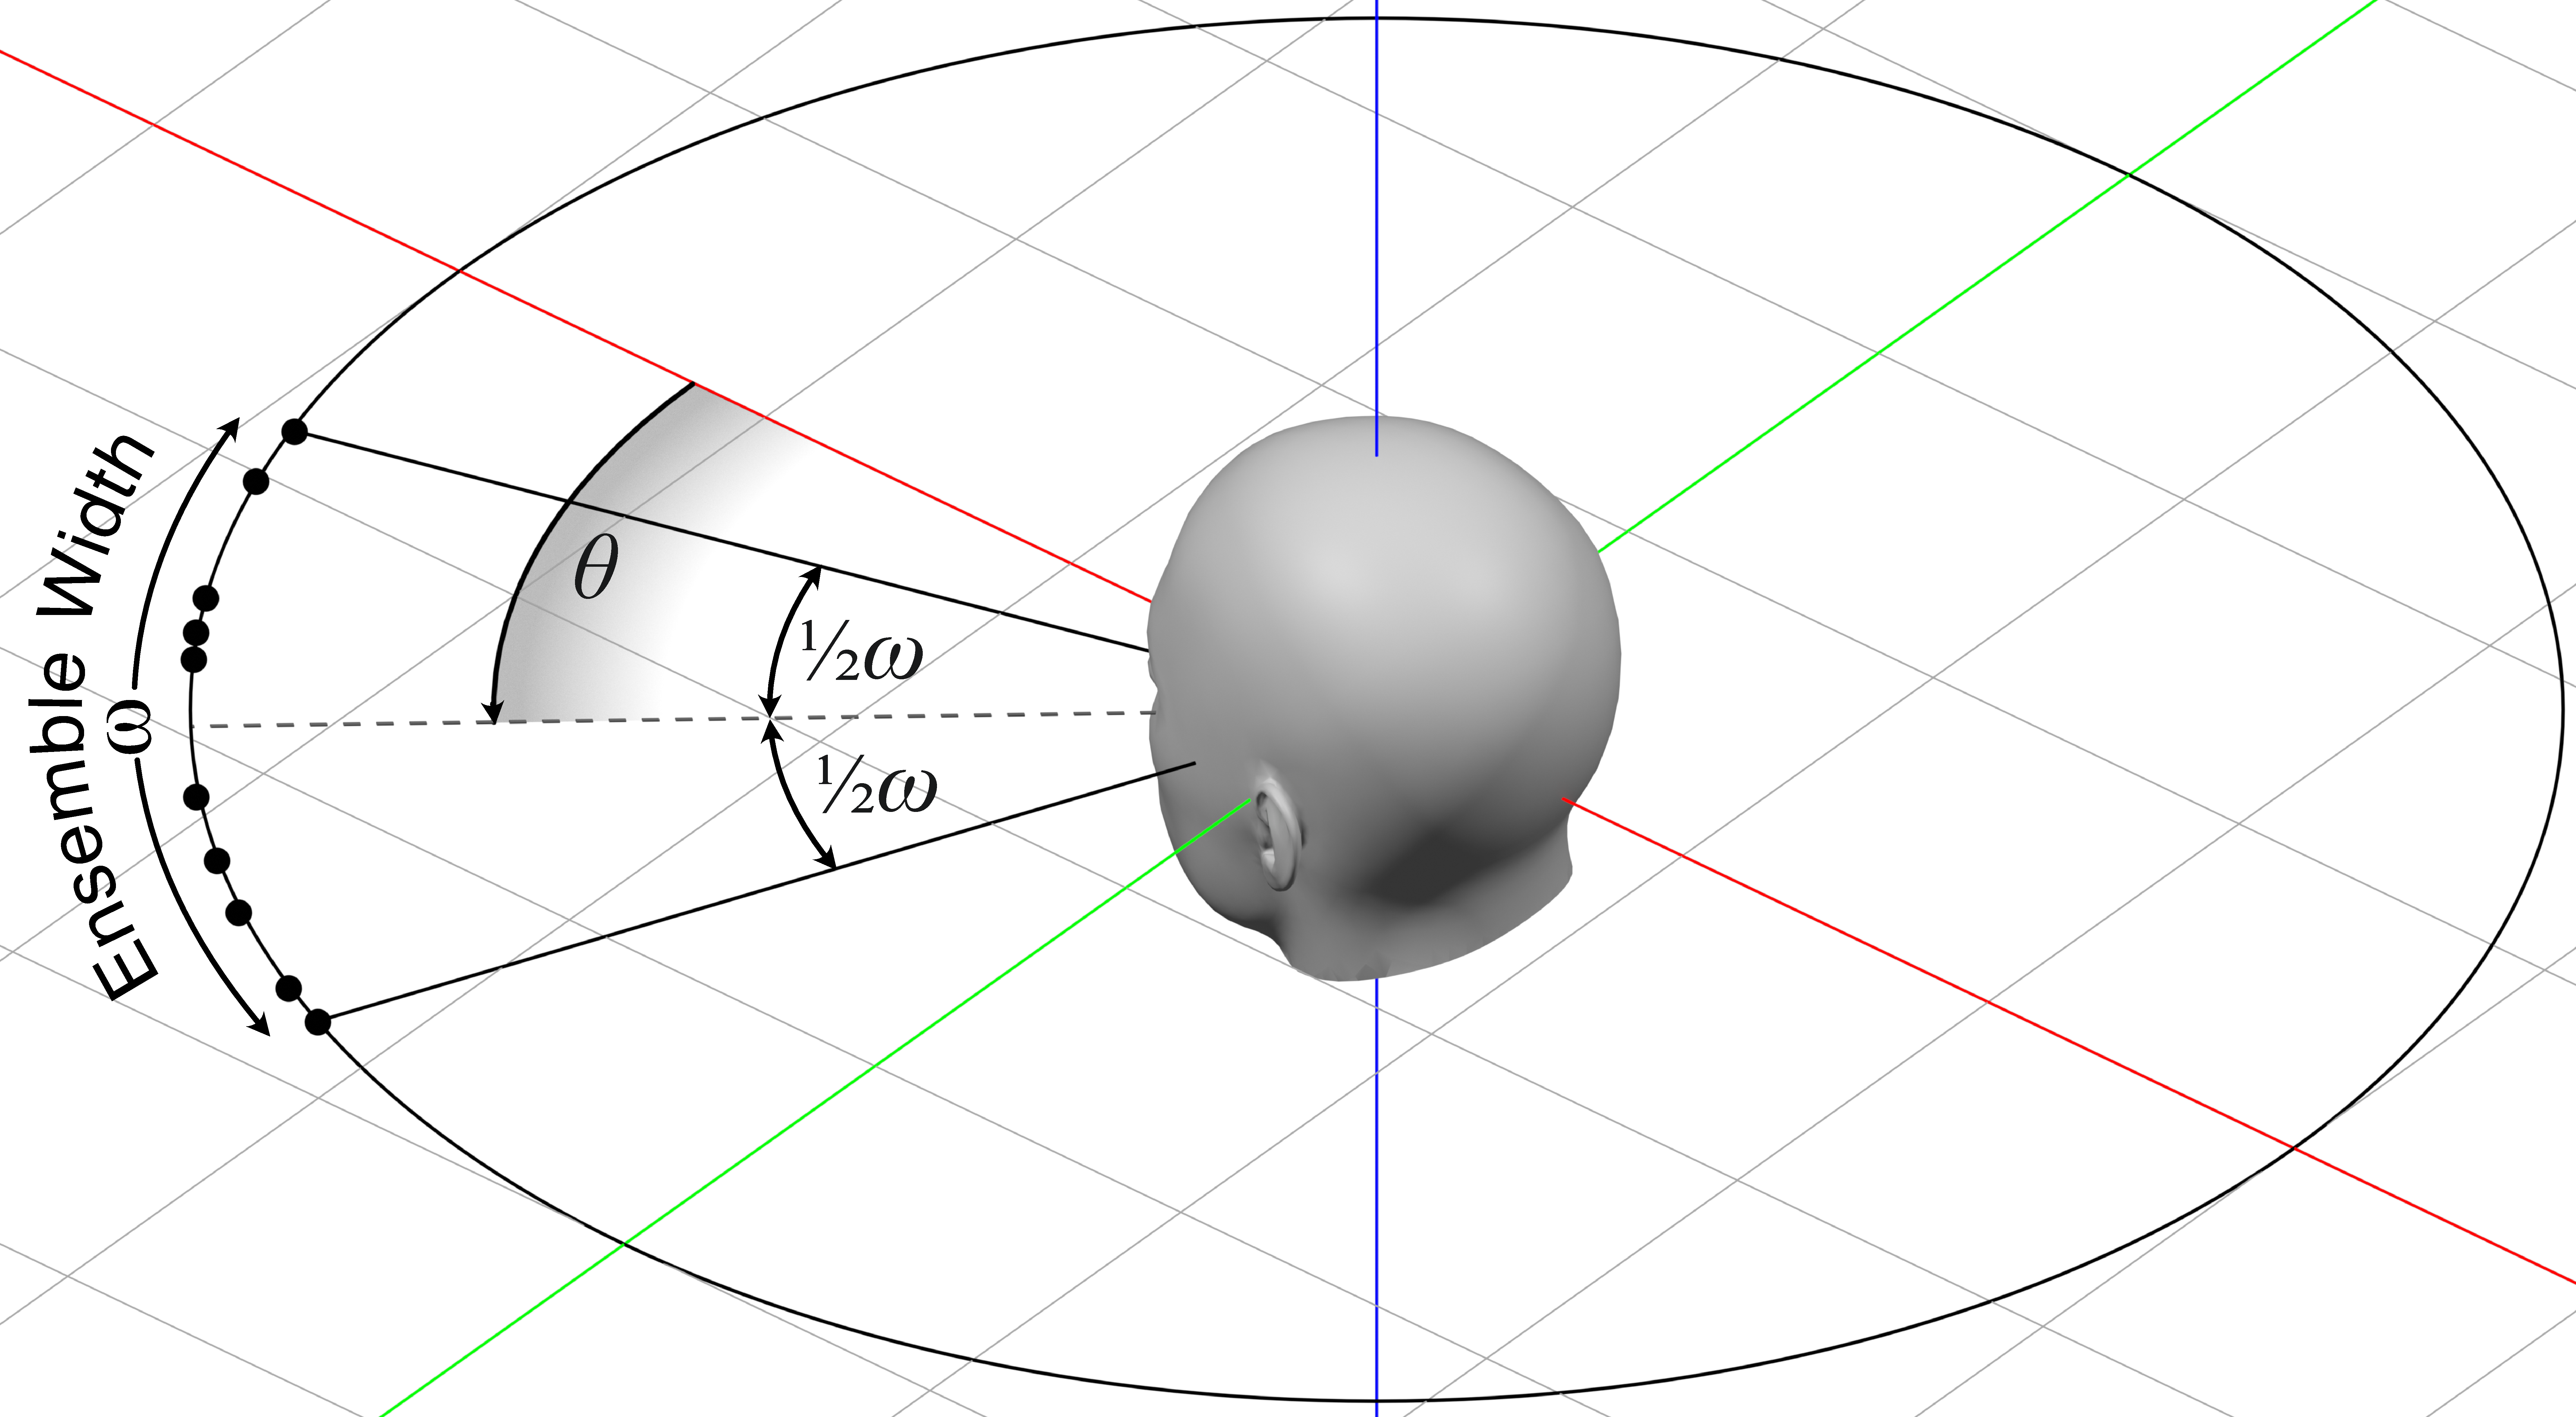
\includegraphics[width=\linewidth]{../pictures/scene2.pdf}
  \caption{\label{fig:scene}Illustration of ensemble width ($\omega$) and ensemble location ($\theta$) relative to the direction of the head orientation. Black dots represent the positions of audio sources $\theta_i$. The ensemble location ($\theta$) is the angular position of the center of the ensemble relative to the direction the head is facing. The ensemble width ($\omega$) is the angular distance between the two most extreme audio sources in the ensemble.}
\end{figure}

The objective of the model developed in this study is to estimate the ensemble location ($\theta$) and width ($\omega$), as illustrated in Figure \ref{fig:scene}. An ensemble is defined as a group of audio point sources positioned on a circle around the listener on a virtual acoustic scene with equal distance to the listener. The location of source $i$ is denoted by $\theta_i$. The ensemble width ($\omega$) is defined as the angular distance between two extreme point sources ($max_i(\theta_i)-min_i(\theta_i)$), while the ensemble location, designated by $\theta$, represents the middle angle between two extreme sound sources ($(max_i(\theta_i)+min_i(\theta_i))/2$). For the purposes of this study, the locations of the sources were limited to the frontal hemisphere only, i.e. $\theta\in[-45\degree, 45\degree]$, $\omega\in[0\degree, 90\degree]$, as this range encompasses the majority of real-world recording scenarios. It should be noted that although humans possess some limited abilities to localize sound sources in the vertical plane, in this study all sources are placed in the horizontal plane, at the ear-level of the listener. This covers the majority of cases for real-world recordings (see \textcite{ma_robust_2018, zielinski_spatial_2022} for related studies that cover top-down discrimination).

\subsection{Synthesis of binaural music recordings}
\label{subsec:synthesis}

The experiments conducted in this study involved 23,040 binaural recordings of music. These recordings were synthesized using 192 publicly-available multi-track music recordings \parencite{senior_mixing_2023} and 30 HRTF databases (see Table \ref{table:hrtfs} in \nameref{appendix:a_hrtf} for a detailed list). The large number of HRTF databases was necessary to make the model as generalizable as possible. In real-world scenarios, the HRTF used for binaural synthesis is often unknown, so constructing a model for a single HRTF would have limited practical utility. The aim was to predict ensemble parameters regardless of the specific HRTF function used. Additionally, the large number of HRTF functions increased the amount of data available for model training, which is particularly beneficial in the context of deep neural networks. The number of HRTF databases (30) was determined using heuristics from previous study conducted by \textcite{zielinski_automatic_2022}, which suggested this number should be sufficient for the task.

The number of tracks in multi-track recording ranged from 5 to 62, with median of 9. For each pair of a multi-track recording and an HRTF database, four binaural recordings were synthesized with different random ensemble parameters, namely location $\theta$ and width $\omega$, as defined in Section \ref{subsec:ensemble_definition}. Both parameters were drawn from a uniform random distribution. Furthermore, the tracks of the input multi-track recordings were randomly assigned to sound source positions ($\theta_i$) to enhance the diversity of the final binaural corpora. Before the synthesis, the signals in each track were equalized to $-23$ LKFS, in accordance with the ITU-R BS.1770-5 (\citeyear{noauthor_itu-r_2023}) recommendation. 

The binaural recordings were obtained in this study using the binaural synthesis procedure, known as binauralization, whose aim was to simulate the positions of sound sources within a virtual acoustic environment \parencite{blauert_spatial_1996}. This was achieved by convolving multi-track signals with head-related impulse responses from a specified head-related transfer function (HRTF) database. The resulting binaural output signal $y_c[n]$ for each stereo channel $c$ (left or right) at sample $n$ is given by the following equation:
\begin{equation}
  y_c[n] = \sum_{i=1}^{N} \sum_{k=0}^{K-1} x_i[k] \times h_{c,\theta_i}[n-k] ,
\end{equation}
where $x_i$ represents the signal of an individual sound source $i$ from the input music recording and $h_{c,\theta_i}$ denotes the head-related impulse response for channel $c$ at location $\theta_i$ of source track $i$.

After the binauralization procedure, the synthesized recordings were truncated to a duration of seven seconds, with sine-squared fade-in and fade-out effects of 0.01 seconds applied. The recordings were then RMS-normalized, scaled by a factor of 0.9, and DC-offset corrected. They were stored as uncompressed files at a 48 kHz sampling rate and with a 32-bit resolution.

Due to copyright restrictions, the music corpus utilized in this study was not published. However, the corpus can be provided upon reasonable request from the authors of this paper.

\subsection{Calculation of spectrograms}
\label{subsec:feature_extraction}

Prior being input into the model, the binaural recordings of music were transformed into magnitude spectrograms. Although spectrograms do not directly provide information that can be translated into ensemble features, especially ensemble width, the goal of this task was to reduce the number of independent variables compared to the raw audio signal by extracting more compressed and informative data in the frequency domain. This step was also necessary to decrease the likelihood of overfitting, reducing the number of examples needed to train the model, and thereby lower the overall computational power requirements. It is worth mentioning, however, that recently published studies have shown that CNNs are suitable for end-to-end audio localization without the spectrogram extraction step, as demonstrated by \textcite{vera-diaz_towards_2018, vecchiotti_end--end_2019}.

To prepare the input for the model, a Hamming window of 40 ms with an overlap of 20 ms was applied to each frame of the signal, resulting in a total of 349 time frames. From each frame, spectrograms were extracted using the Fast Fourier Transform (FFT) algorithm, with 150 frequency bands spaced linearly from 100 Hz to 16 kHz. This procedure was conducted for both the left and right channels, yielding two spectrograms for each binaural sample. Consequently, each sample was represented by a 32-bit floating-point precision matrix of dimensions $2 \times 349 \times 150$. This method parallels the procedure presented by \textcite{zielinski_automatic_2022}.

\subsection{Network topology}
\label{subsec:topology}

The network topology employed in this study was strongly influenced by the AlexNet convolutional neural network introduced by \textcite{krizhevsky_imagenet_2012}. While AlexNet was originally designed for image classification, in this study it was adapted for the audio analysis task by converting binaural recordings into magnitude spectrograms, as described in Section \ref{subsec:feature_extraction}. This conversion allowed the spectrograms to be treated like visual data, enabling them to be used in an image-recognition-like task.

As illustrated in Figure \ref{fig:architecture}, the network architecture consists of an input layer accepting a pair of spectrograms, followed by a series of convolutional units and classification units, culminating in two outputs predicting ensemble location and width, respectively. This design employs a multi-task approach, enabling a single network to estimate both ensemble parameters simultaneously.

\begin{figure}[ht!]
  \centering
  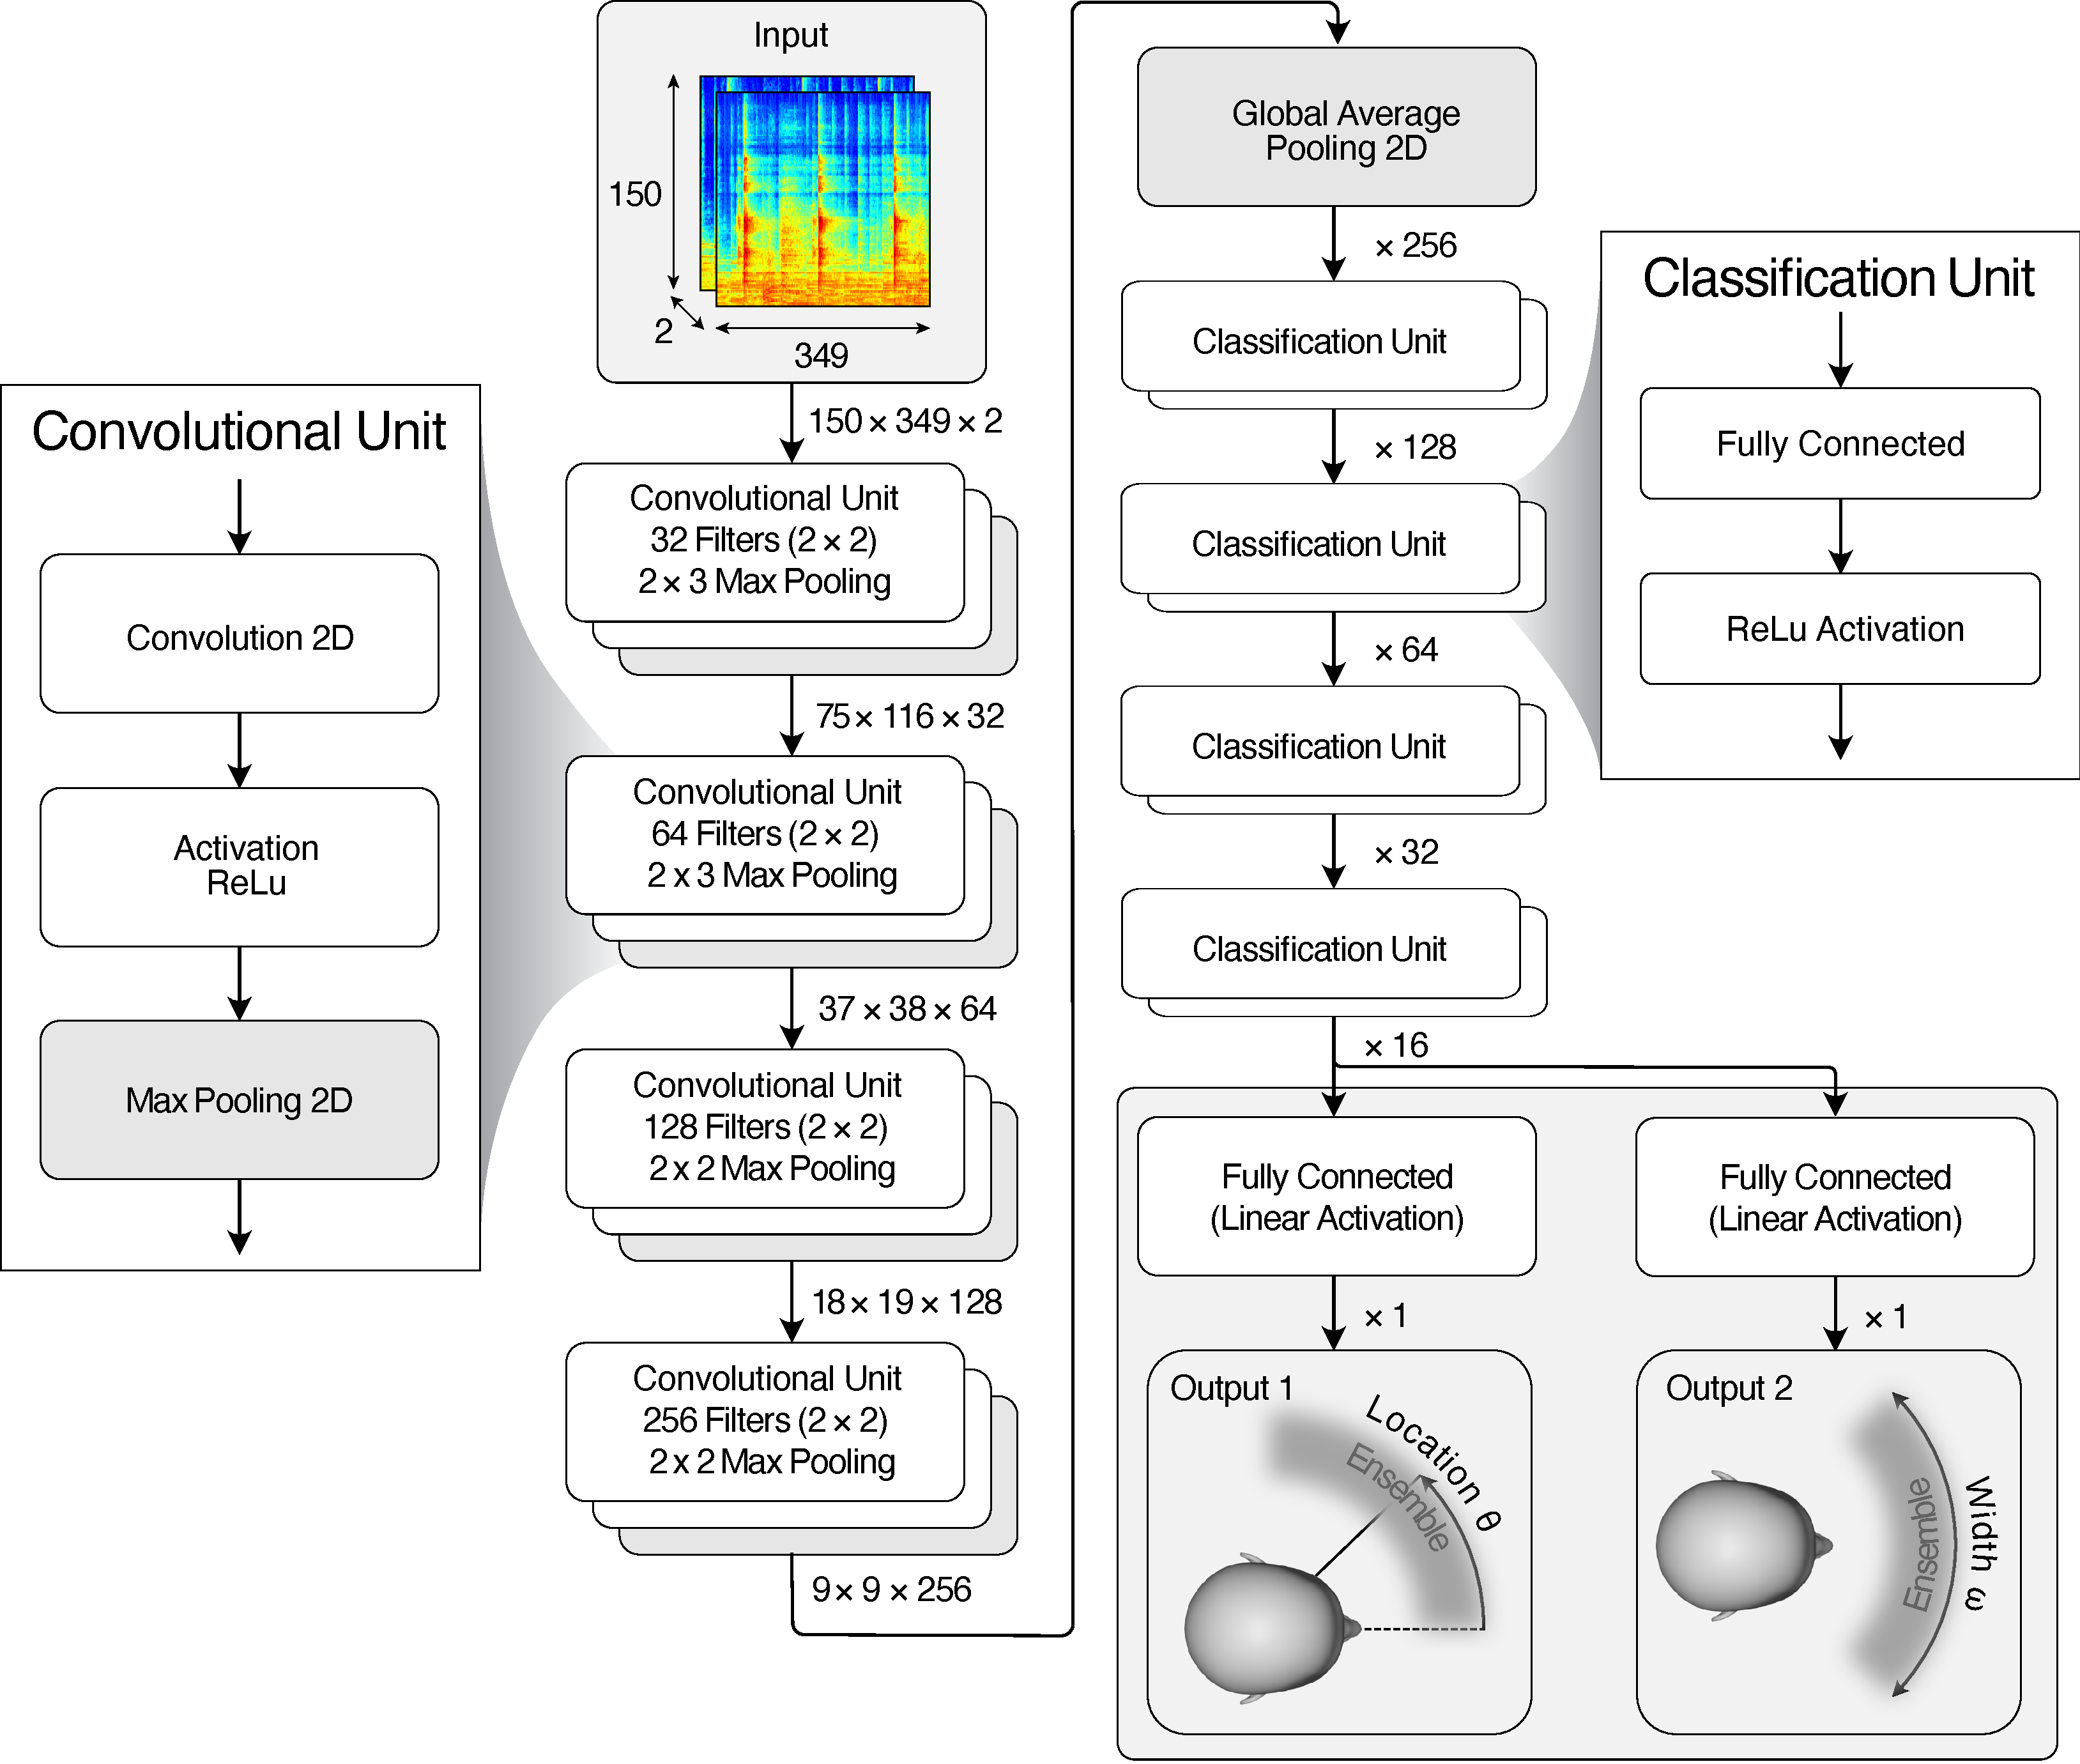
\includegraphics[width=\linewidth]{../pictures/architecture.pdf}
  \caption{\label{fig:architecture}Topology of the Convolutional Neural Network (CNN) used for estimating ensemble location and width, illustrating the layers (grouped in ``convolutional'' and ``classification'' units) and connections of the network architecture.}
\end{figure}

The topology finalized in this study was chosen, among many alternative architectures, based on the highest prediction quality observed on the validation dataset. Despite the existence of numerous algorithms for automatic topology selection \parencite{branke_evolutionary_1995, zhang_finding_2018, miikkulainen_evolving_2017, stanley_evolving_2002, shafiee_deep_2016}, the final topology was determined manually, primarily due to the high computational demands relative to the available resources.

Various architectural configurations were assessed, with key parameters being varied such as the number of convolutional units (from 1 to 5), the number of classification units (from 1 to 5), the inclusion or exclusion of max pooling layers after each convolution layer, the number of filters within the convolutional layers, the dimensions of these filters ($2 \times 2$, $2 \times 3$, or $3 \times 3$), the stride size, and the dimensions of the max pooling layers ($2 \times 2$, $2 \times 3$, or $3 \times 3$). Based on this procedure, it was concluded that the model is robust against variations in the assessed topologies. The differences in mean prediction error among the configurations were minimal, typically less than $1\degree$ for most configurations. Among the many tested topologies that yielded similar errors, the simplest one was selected to optimize both performance efficiency and model simplicity.

Despite the availability of widely used techniques for addressing  an overfitting effect, such as the dropout layer \parencite{srivastava_dropout_2014}, and for accelerating training, such as batch normalization \parencite{ioffe_batch_2015}, neither technique was employed in this study as they were observed to be ineffective for the specific estimation task being undertaken. Instead, a global average pooling layer was utilized, known for its capabilities in reducing overfitting \parencite{lin_network_2013}. This was confirmed in this particular task, as the inclusion of this layer significantly reduced overfitting, lowering the final mean absolute error (MAE) score by $0.83\degree$ (average across 10 trials) compared to configurations where a simple flattening layer was used instead.

\subsection{Model training and evaluation}
\label{subsec:training_evaluation}

The topology described in the previous section resulted in a model with 216,562 learning parameters. The model training procedure was repeated 10 times, employing the Monte Carlo cross-validation method, as described by \textcite{kuhn_applied_2013}. For each repetition, the entire dataset was randomly divided into two parts: a development set containing two-thirds of the dataset (15,360 recordings) for model construction, and a test set consisting of the remaining one-third of the dataset (7,680 recordings) for its evaluation. This repetition procedure was employed to ensure more reliable and generalizable results by assessing the model's performance across different subsets of the data. Additionally, it helped to account for the inherent variability in neural network training, where slight changes in initial conditions or optimization paths can lead to different model outcomes. While a large and diverse dataset could mitigate this issue, the binaural excerpts used in this study were generated from only 196 multi-track music recordings. This limited source material raised concerns by these authors about potential significant variations between the development and test sets in each repetition. In hindsight, these concerns were valid, as the maximum observed difference in MAE between repetitions reached up to $0.85\degree$ for ensemble width.

To ensure that the evaluation process was unbiased, the data split was done in such a way that no original multi-track recordings used for synthesis were included in both the development and test sets simultaneously. However, this rule was not applied to HRTFs databases, allowing for the possibility of HRTF information leaking between the development and test sets. This could be seen as a significant limitation of the study. However, it is known that a human auditory system uses a single HRTF represented by ears, head, and torso, only slightly changing throughout the entire life, mainly during infancy \parencite{clifton_growth_1988, king_how_2001}. Therefore, this limitation could be considered in pair how the human auditory system behaves in real life. Nevertheless, it is worth noting that some studies implement HRTF-independent testing for binaural localization models, as demonstrated by \textcite{zielinski_spatial_2022, zielinski_automatic_2022,antoniuk_blind_2023}.

The development set was divided into training and validation subsets at a 7:1 ratio, with 13,440 recordings in the training subset and 1,920 recordings in the validation subset. The training subset was used to update the model's learning parameters, while the validation subset was solely used for early stopping \parencite{pocock_practical_1989, morgan_generalization_1989} and model checkpointing \parencite{eisenman_check-n-run_2020}. These techniques were employed to select the model with the best generalization capabilities and prevent overfitting. The test subset, which included data not seen during the training or validation phases, was used solely for performance assessment once per a repetition. This divide-train-and-evaluate process was repeated to collect 10 mean absolute errors, from which the final model error was determined.

For each sample, the model received two spectrograms as input: one for the left channel and one for the right channel. The rationale behind the application of Convolutional Neural Networks (CNNs) to this task was to automatically extract local features from the spectrograms and use these features to estimate two contiguous ensemble parameters: ensemble location and width, both measured in degrees. For model training, the Adam algorithm \parencite{kingma_adam_2014} was used. The algorithm minimized prediction errors, calculated as the difference between the actual ensemble parameters (known \textit{a priori} from the binaural synthesis described in Section \ref{subsec:synthesis}) and the predicted values.

The optimizer was configured with the following hyperparameters: an initial learning rate of $10^{-3}$, a decay rate of $10^{-6}$, and momentum parameters $\beta_1 = 0.9$ and $\beta_2 = 0.999$. Training was conducted using a batch size of 8, with a maximum of 256 epochs set. An early stopping technique was implemented to prevent overfitting, terminating the process if no improvement was observed on the validation set for 20 consecutive epochs. Consequently, the maximum number of epochs was never reached; instead, training concluded after 25 to 36 epochs, with a median of 27.5 epochs. During the training process, the losses for both outputs were combined additively, ensuring equal weighting of both ensemble features.

The computational work for this study was conducted on a workstation equipped with an RTX Nvidia GeForce 4090 GPU and a 48-core AMD Ryzen ThreadRipper processor (up to 4.5 GHz). On the software side, MATLAB \parencite{MATLAB} with the Audio Toolbox \parencite{MATLAB_Audio_Toolbox} was used for the binaural recording synthesis, while Python \parencite{python} with the SciPy package \parencite{2020SciPy-NMeth} was used for feature extraction and Keras \parencite{chollet_keras_2015} for training the CNN model. The complete source code for all the experimental stages is publicly available on the GitHub repository \parencite{antoniuk_software_2024}. The spectrogram calculation phase required 21 minutes, data partitioning took 34 minutes, and the total training time for all iterations amounted to 40 minutes, making the entire training and evaluation process 95 minutes long.

\section{Results and discussion}
\label{sec:results}

The overall model performance measured across 10 experiment iterations, expressed as mean absolute error (MAE), was equal to $8.57\degree$ ($\pm0.19\degree$) for ensemble width and $4.76\degree$ ($\pm0.10\degree$) for ensemble location. As both ensemble parameters were constrained within the same range of $90\degree$, the results demonstrate that the model exhibits a $44\%$ lower error for ensemble location compared to ensemble width. This outcome is not unexpected, given that ensemble location is a less complex parameter. Essentially, it represents the average location of all sources. Therefore, it is more resistant to temporal fluctuations in individual audio sources than ensemble width, which is dependent on the two most extreme sound sources that vary over time. Furthermore, estimating ensemble width necessitates the identification of these two extreme sources, a process that is inherently more complex than estimating a single average location.

Figure \ref{fig:actual_vs_predicted_width} compares the actual and predicted ensemble widths for each sample, showing a heteroscedastic relationship between them, with a slight bias towards predicting lower ensemble width values for higher actual widths. This relationship exhibits a strong positive correlation, with a Pearson coefficient $r$ of 0.90. Additionally, the results indicate that the model provides more precise predictions for narrower ensemble widths, with an average MAE of $5.65^\circ$ for $\omega < 30^\circ$. However, performance deteriorates as the ensemble width increases, resulting in an MAE of $12.44^\circ$ for $\omega > 80^\circ$. This effect is more visible in Figure \ref{fig:mae_width}, which highlights the impact of the actual ensemble width on the precision of prediction. The correlation between the actual ensemble width and prediction error shows a weak positive relationship, with a Pearson coefficient $r$ of 0.27.

\begin{figure}[ht!]
  \centering
  \begin{minipage}[]{0.45\linewidth}
    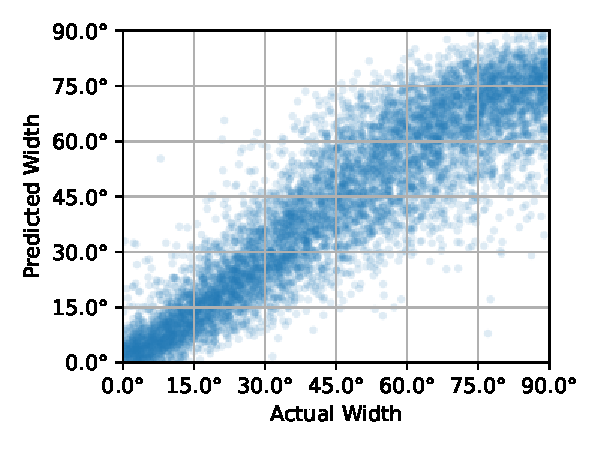
\includegraphics[width=\linewidth]{../figures/actual_vs_predicted_width.pdf}
    \caption{\label{fig:actual_vs_predicted_width}A comparison between the actual ensemble width $\omega$ and the predicted ensemble width $\omega'$ for a single iteration (of the total ten). }
  \end{minipage}
  \hspace{0.5cm}
  \begin{minipage}[]{0.45\linewidth}
    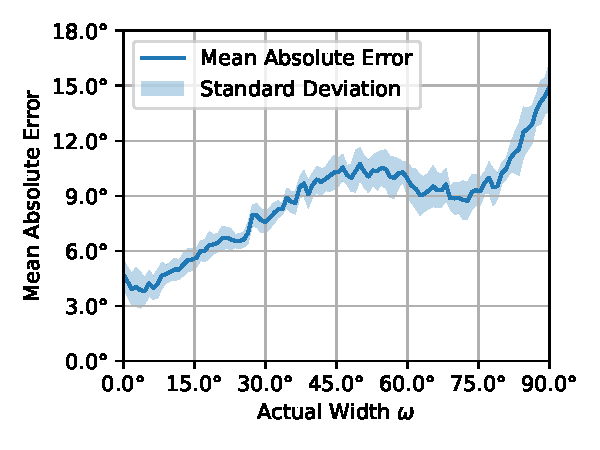
\includegraphics[width=\linewidth]{../figures/mae_width.pdf}
    \caption{\label{fig:mae_width}The impact of the actual ensemble width $\omega$ on the mean absolute prediction error, averaged across all ten iterations, with indicated standard deviation.}
  \end{minipage}
\end{figure}

The reduced accuracy in the width prediction can be attributed to the sparse distribution of audio sources in wider ensembles, which amplifies the influence of extreme sound sources on prediction errors, resulting in lower precision as the ensemble width increases. Moreover, Figure \ref{fig:mae_width} reveals that the relationship between the ensemble width and the error is nonlinear, displaying a notable decrease in error between $60\degree$ and $75\degree$. The reason for this nonlinearity is currently unclear and requires further investigation.

The correlation between the actual and predicted ensemble location values exhibits a very high degree of correlation, as illustrated in Figure \ref{fig:actual_vs_predicted_location}. In this case, Pearson correlation coefficient $r$ is equal to as much as 0.97. In contrast to the ensemble width, no significant relationship is observed between actual location and its prediction error. This finding suggests that the model's ability to localize the center of the ensemble is robust, unaffected by the actual spatial positioning of the ensemble, including lateral locations. Figure \ref{fig:mae_location} corroborates this observation, demonstrating relatively consistent location error across most positions, with minor increases at extreme locations. The negligible correlation ($r = -0.03$) between the absolute location value and prediction error further supports the model's spatial invariance in its performance.

\begin{figure}[ht!]
  \centering
  \begin{minipage}[t]{0.45\linewidth}
    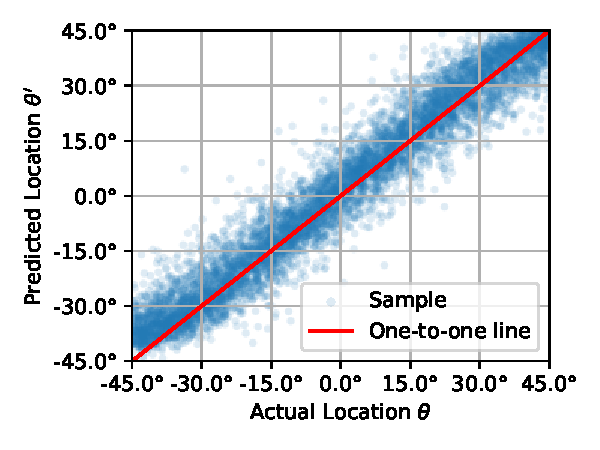
\includegraphics[width=\linewidth]{../figures/actual_vs_predicted_location.pdf}
    \caption{\label{fig:actual_vs_predicted_location}A comparison between the actual ensemble location $\theta$ and the predicted ensemble location $\theta'$ for a single iteration (of the total ten) }
  \end{minipage}
  \hspace{0.5cm}
  \begin{minipage}[t]{0.45\linewidth}
    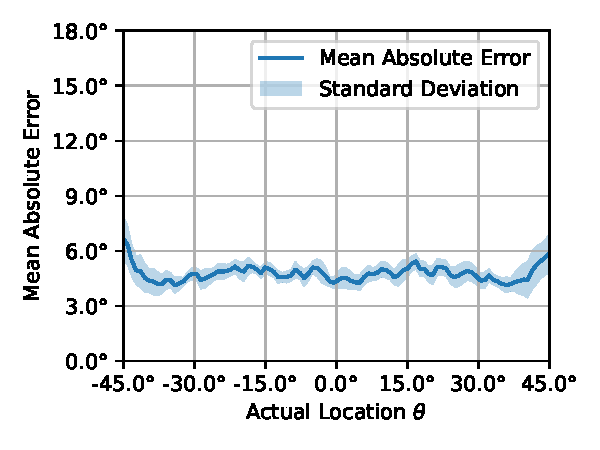
\includegraphics[width=\linewidth]{../figures/mae_location.pdf}
    \caption{\label{fig:mae_location}The impact of the actual ensemble width $\omega$ on the mean absolute prediction error, averaged across all ten iterations, with indicated standard deviation.}
  \end{minipage}
\end{figure}

Figure \ref{fig:map_mae_location} illustrates the influence of both ensemble location and width on the mean absolute error for ensemble location, providing a detailed perspective complementing the results presented in Figure \ref{fig:mae_location}. Notably, the figure highlights asymmetric anomalies, particularly within the $\theta \in [15\degree, 30\degree]$ range compared to the $\theta \in [-30\degree, -15\degree]$ range, which can be attributed to the sparsity of sample result data across specific regions of this heatmap. While the figure suggests that ensemble location does not significantly affect the model's precision in predicting location, it clearly demonstrates that ensemble width has a substantial impact. Specifically, there is a positive correlation between the width of the ensemble and the error in its location prediction, with error magnitude increasing as the width expands.

\begin{figure}[ht!]
  \centering
  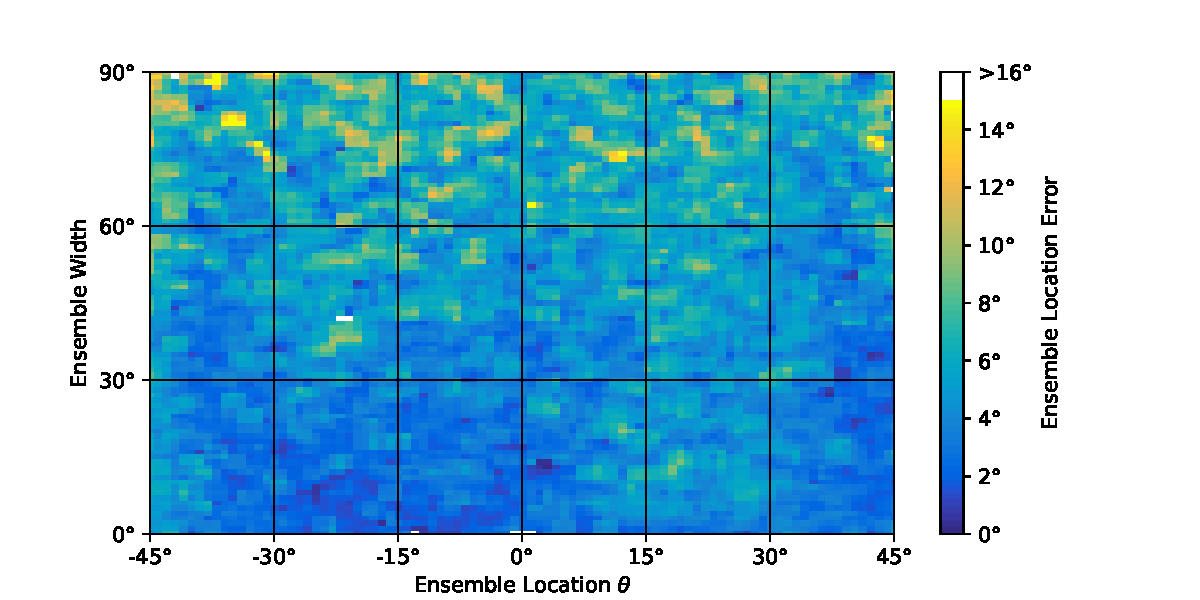
\includegraphics[width=\linewidth]{../figures/map_mae_location.pdf}
  \caption{\label{fig:map_mae_location}The heatmap illustrating the mean absolute error (MAE) of ensemble location distribution across different ensemble locations (x-axis) and ensemble widths (y-axis). The color intensity corresponds to the MAE values, with lighter areas indicating higher errors.}
\end{figure}

Figure \ref{fig:map_mae_width} reveals a characteristic performance depression in $\omega \in [30\degree, 60\degree]$ previously shown from a different perspective in Figure \ref{fig:mae_width}. This heatmap highlights another interesting phenomenon in its upper corners as the error in these areas is considerably higher. This indicates that the model's performance for estimating ensemble width is substantially worse at extreme widths and locations, i.e., when both the width and locations are near their maximum investigated values ($|\theta| \approx 45\degree, \omega \approx 90\degree$).

\begin{figure}[ht!]
  \centering
  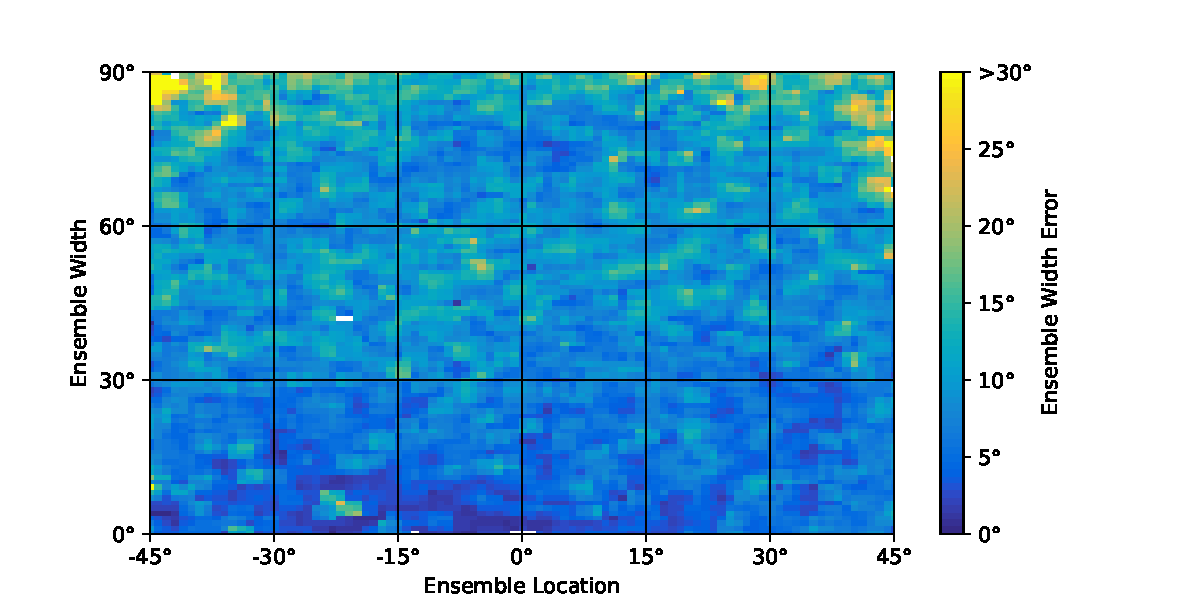
\includegraphics[width=\linewidth]{../figures/map_mae_width.pdf}
  \caption{\label{fig:map_mae_width}The heatmap illustrating the mean absolute error (MAE) of ensemble width distribution across different ensemble locations (x-axis) and ensemble widths (y-axis). The color intensity corresponds to the MAE values, with lighter areas indicating higher errors.}
\end{figure}

The model presented in this study demonstrates a significant improvement in ensemble-width performance compared to the Spatiogram-based model, first introduced by \textcite{arthi_spatiogram_2021} and further investigated by \textcite{antoniuk_blind_2023}, under similar evaluation conditions. While the dataset used in this study was expanded with 40 additional multi-track recordings and 10 HRTF databases, \textcite{antoniuk_blind_2023} showed that the Spatiogram model's performance does not improve with further increases in dataset size. This finding enables a direct comparison of results between the two models in terms of the precision of the ensemble width estimation, despite the differences in dataset composition. Our model achieved a MAE of $8.57\degree$, outperforming the Spatiogram-based model's result of $13.62\degree$ by $5.05\degree$. This substantial improvement is further enhanced by the current model's ability to estimate ensemble location, a feature absent in the previous model.

In terms of ensemble location prediction, the novelty of the proposed method makes direct comparison with existing literature challenging. However, its efficacy can be only evaluated indirectly against state-of-the-art individual-source localization techniques. The ensemble location prediction precision (MAE $=4.76\degree$) of the proposed method can be contextualized with the leading-edge binaural localization DeepEar model introduced by \textcite{yang_deepear_2022}. Their model reported MAEs of $7.4\degree$ and $2.3\degree$ for multi-source and single-source Angle of Arrival (AoA) estimation, respectively. As another promising example, the WaveLoc-CONV model developed by \textcite{vecchiotti_end--end_2019} demonstrated errors of $0\degree$ in anechoic conditions and $1.7\degree-2.4\degree$ in multi-condition scenarios. However, these results are limited to single-source speech localization, a substantially less complex task than the ensemble location prediction addressed by the proposed method. These experiments, while differing in objectives and datasets, provide valuable context for the proposed method's performance within current DoA and AoA estimation research.

\section{Conclusions}
\label{sec:conclusions}

This paper introduces a novel approach to locating audio sources in binaural recordings. Unlike traditional methods that predict the locations of individual audio sources, this study focuses on estimating ``ensemble parameters'' of audio sources, thus allowing the audio scene to be described using two parameters only: ensemble location and width. This approach makes it possible to avoid making restrictive assumptions about the number of audio sources, rendering the proposed method more suitable for real-world applications. The study also explores the use of convolutional neural networks (CNN) in conjunction with spectrograms applied to their inputs. According to the obtained results, the networks show exceptionally good performance, demonstrating their suitability for the investigated scenario.

The method was developed using 23,040 synthesized binaural excerpts intended to mimic real-world music recordings. The results show its outstanding performance, with the model achieving mean absolute error (MAE) of $4.76\degree \pm 0.10\degree$ and $8.57\degree \pm 0.19\degree$ for the estimation of ensemble location and width, respectively. While the model is resilient to lateral ensemble locations, it is sensitive to the actual ensemble width, lowering the model accuracy as the width increases. The proposed method demonstrates a significant improvement over the previous technique based on spatiograms \parencite{antoniuk_blind_2023}, lowering the mean absolute error by $5.05\degree$.

Despite its high precision, the method exhibits certain limitations. Since it has been developed using the binaural excerpts synthesized with the head-related impulse responses being inherently anechoic in their characteristics, the method's performance under reverberant conditions has not been validated. Moreover, the proposed method is incapable of operating in real-time scenarios. Validating the method under reverberant conditions as well as optimizing its architecture for practical real-time scenarios constitute the topics for future research. Other minor limitations include the lack of head-related transfer-function (HRTF) independence between the development and test sets, and the absence of vertical variations in audio source placement, as all sources were positioned on the horizontal plane. Additionally, the proposed approach requires substantial computational resources, particularly GPU usage, which was not necessary for the previously used spatiogram-based method.

These limitations, however, present opportunities for future research. Despite the current constraints, this study introduces a novel method for characterizing acoustic scenes in binaural recordings of music, demonstrating substantial potential for advancing binaural audio analysis. The method offers promising prospects for developing innovative tools that can objectively analyze large repositories of binaural audio recordings, focusing on spatial content.

% \clearpage
\section*{Acknowledgments}
The work was supported by the grants from Białystok University of Technology (WI/WI-IIT/3/2022 and WZ/WI-IIT/5/2023) and funded with resources for research by the Ministry of Science and Higher Education in Poland.

\section*{Appendix}
\label{appendix:a_hrtf}

\begin{longtblr}[
  caption = {List of HRTF sets used to synthesize binaural audio excerpts},
  label = {table:hrtfs}
  ]{
  colspec={c|c|>{\raggedright\arraybackslash}X|c|>{\raggedright\arraybackslash}X|c},
  hlines = {},
  vlines = {},
  cell{2}{5} = {r=2}{m},
  cell{2}{6} = {r=2}{m},
  cell{4}{5} = {r=4}{m},
  cell{4}{6} = {r=4}{m},
  cell{8}{5} = {r=3}{m},
  cell{8}{6} = {r=3}{m},
  cell{11}{6} = {r=2}{m},
  cell{13}{5} = {r=3}{m},
  cell{13}{6} = {r=3}{m},
  cell{16}{5} = {r=2}{m},
  cell{16}{6} = {r=2}{m},
  cell{18}{5} = {r=2}{m},
  cell{18}{6} = {r=2}{m},
  cell{20}{5} = {r=3}{m},
  cell{20}{6} = {r=3}{m},
  cell{23}{5} = {r=3}{m},
  cell{23}{6} = {r=3}{m},
  cell{28}{5} = {r=2}{m},
  cell{28}{6} = {r=2}{m},
  cell{30}{5} = {r=2}{m},
  cell{30}{6} = {r=2}{m},
  }
  \textbf{No.} & \textbf{Type} & \textbf{Head}                             & \textbf{Radius {[}m{]}} & \textbf{Source}                                                                                                                            & \textbf{Acronym} \\*
  1.           & Human         & Human subject                             & 1.2                     & RWTH Aachen University \parencite{braren_high-resolution_2020}                                                                             & AACHEN           \\*
  2.           & Artificial    & GRAS 45BB-4 KEMAR                         & 1                       &                                                                                                                                            &                  \\
  3.           & Human         & Subject 2                                 & 1.2                     & Austrian Academy of Sciences \parencite{noauthor_hrtf-database_2014}                                                                       & ARI              \\*
  4.           & Human         & Subject 4                                 & 1.2                     &                                                                                                                                            &                  \\*
  5.           & Human         & Subject 10                                & 1.2                     &                                                                                                                                            &                  \\*
  6.           & Artificial    & ARI Printed Head                          & 1.2                     &                                                                                                                                            &                  \\
  7.           & Human         & Subject 012                               & 1                       & CIPIC Interface Laboratory, University of California \parencite{algazi_cipic_2001}                                                         & CIPIC            \\*
  8.           & Human         & Subject 015                               & 1                       &                                                                                                                                            &                  \\*
  9.           & Human         & Subject 020                               & 1                       &                                                                                                                                            &                  \\
  10.          & Artificial    & Neumann KU 100                            & 0.9                     & NASA (2007) \parencite{andreopoulou_inter-laboratory_2015}                                                                                 & CLUBFRITZ        \\*
  11.          & Artificial    & Neumann KU 100                            & 1.5                     & Helsinki University of Technology (2009) \parencite{andreopoulou_inter-laboratory_2015}                                                    &                  \\
  12.          & Artificial    & FABIAN                                    & 1.47                    & Technical University Berlin, Huawei Technologies, Munich Research Centre, Sennheiser Electronic \parencite{brinkmann_cross-evaluated_2019} & HUTUBS           \\*
  13.          & Human         & Subject pp2                               & 1.47                    &                                                                                                                                            &                  \\*
  14.          & Human         & Subject pp3                               & 1.47                    &                                                                                                                                            &                  \\
  15.          & Human         & Subject 1003                              & 1.95                    & IRCAM, AKG \parencite{noauthor_listen_2023}                                                                                                & LISTEN           \\*
  16.          & Human         & Subject 1002                              & 1.95                    &                                                                                                                                            &                  \\
  17.          & Artificial    & KEMAR DB-4004 (DB-061)                    & 1.4                     & MIT \parencite{gardne_hrtf_1994}                                                                                                           & MIT              \\*
  18.          & Artificial    & KEMAR DB-4004 (DB-065)                    & 1.4                     &                                                                                                                                            &                  \\
  19.          & Human         & Subject 001                               & 1.5                     & Tohoku University \parencite{watanabe_dataset_2014}                                                                                        & RIEC             \\*
  20.          & Human         & Subject 002                               & 1.5                     &                                                                                                                                            &                  \\*
  21.          & Artificial    & Koken SAMRAI                              & 1.5                     &                                                                                                                                            &                  \\
  22.          & Artificial    & Neumann KU 100                            & 1.2                     & University of York \parencite{armstrong_perceptual_2018}                                                                                   & SADIE II         \\*
  23.          & Human         & Subject H3                                & 1.2                     &                                                                                                                                            &                  \\*
  24.          & Human         & Subject H4                                & 1.2                     &                                                                                                                                            &                  \\
  25.          & Artificial    & KEMAR                                     & 1                       & South China University of Technology \parencite{yu_near-field_2018}                                                                        & SSCUT            \\
  26.          & Artificial    & Neumann KU 100                            & 1                       & TH Köln  \parencite{porschmann_spherical_2017}                                                                                             & STH Köln         \\
  27.          & Artificial    & FABIAN                                    & 1.7                     & TU Berlin \parencite{brinkmann_high_2017, wierstorf_free_2011}                                                                             & TU Berlin        \\*
  28.          & Artificial    & GRAS 45BA KEMAR                           & 1                       &                                                                                                                                            &                  \\
  29.          & Artificial    & GRAS 45BB-4 KEMAR - subject A attachment  & 1                       & Aalborg University; University of Iceland \newline \parencite{spagnol_viking_2019,spagnol_viking_2020}                                     & VIKING           \\*
  30.          & Artificial    & GRAS 45BB-4 KEMAR - subject B attachments & 1                       &                                                                                                                                            &                  \\
\end{longtblr}

\printbibliography

\end{document}

